% !TEX TS-program = pdfLaTeX+MakeIndex+BibTeX
% !TEX encoding = UTF-8 Unicode

\PassOptionsToPackage{unicode}{hyperref}
\PassOptionsToPackage{naturalnames}{hyperref}

\documentclass[tg]{mdtufsm}

\usepackage[T1]{fontenc}
\usepackage{fix-cm}
\usepackage{times, color}
\usepackage[utf8]{inputenc}
\usepackage{graphicx}
\usepackage{amsmath,latexsym,amssymb}
%\usepackage[hidelinks]{hyperref}
\usepackage[hidelinks,
            bookmarksopen=true,linktoc=none,colorlinks=true,
            linkcolor=black,citecolor=black,filecolor=magenta,urlcolor=blue,
            pdftitle={Exploração da Linguagem Rust para o Desenvolvimento de um Path Tracer Paralelo},
            pdfauthor={Yuri Kunde Schlesner},
            pdfsubject={Trabalho de Graduação},
            pdfkeywords={Computação de alto desempenho, programação web, Programação Paralela, Rust, Path Tracing, Informática, UFSM}
            ]{hyperref}
%\usepackage[brazilian]{babel}

%\usepackage{fontspec}
%\setmainfont{Linux Libertine G}

%%% PAGE DIMENSIONS
\usepackage[inner=30mm,outer=20mm,top=30mm,bottom=20mm]{geometry} 
\usepackage{epstopdf}
\usepackage{graphicx}
% \geometry{margin=2in} % for example, change the margins to 2 inches all round
% \geometry{landscape} % set up the page for landscape

% \usepackage[parfill]{parskip} % Activate to begin paragraphs with an empty line rather than an indent

%%% PACKAGES
%\usepackage{amsfonts}
%\usepackage{color}
%\usepackage{booktabs} % for much better looking tables
%\usepackage{array} % for better arrays (eg matrices) in maths
%\usepackage{paralist} % very flexible & customisable lists (eg. enumerate/itemize, etc.)
\usepackage{verbatim} % adds environment for commenting out blocks of text & for better verbatim
\usepackage{listings}
\usepackage{parcolumns}
%\usepackage{microtype}
%\usepackage[numbers]{natbib}
%\usepackage{subfig} % make it possible to include more than one captioned figure/table in a single float
% These packages are all incorporated in the memoir class to one degree or another...

\lstset{
	basicstyle=\scriptsize\ttfamily,
	tabsize=2,
	frame=single,
	breaklines=true,
	breakatwhitespace=true,
	xleftmargin=0cm,
	xrightmargin=0cm,
	literate=
		{á}{{\'a}}1 {é}{{\'e}}1 {í}{{\'i}}1 {ó}{{\'o}}1 {ú}{{\'u}}1
		{Á}{{\'A}}1 {É}{{\'E}}1 {Í}{{\'I}}1 {Ó}{{\'O}}1 {Ú}{{\'U}}1
		{à}{{\`a}}1 {è}{{\`e}}1 {ì}{{\`i}}1 {ò}{{\`o}}1 {ù}{{\`u}}1
		{À}{{\`A}}1 {È}{{\'E}}1 {Ì}{{\`I}}1 {Ò}{{\`O}}1 {Ù}{{\`U}}1
		{ä}{{\"a}}1 {ë}{{\"e}}1 {ï}{{\"i}}1 {ö}{{\"o}}1 {ü}{{\"u}}1
		{Ä}{{\"A}}1 {Ë}{{\"E}}1 {Ï}{{\"I}}1 {Ö}{{\"O}}1 {Ü}{{\"U}}1
		{â}{{\^a}}1 {ê}{{\^e}}1 {î}{{\^i}}1 {ô}{{\^o}}1 {û}{{\^u}}1
		{Â}{{\^A}}1 {Ê}{{\^E}}1 {Î}{{\^I}}1 {Ô}{{\^O}}1 {Û}{{\^U}}1
		{ã}{{\~a}}1 {Ã}{{\~A}}1
		{ç}{{\c c}}1 {Ç}{{\c C}}1
}

% For Computer Modern:
%\def\Cpp{{C\nolinebreak[4]\hspace{-.05em}\raisebox{.4ex}{\tiny\bf ++}}}
% For Linux Libertine G
\def\Cpp{{C\nolinebreak[4]\raisebox{.20ex}{\small\bf++}}}

\newcommand{\todo}[1]{\textsf{\color{red}#1}}


%%=============================================================================
%% Trampa para corrigir o bug do hyperref que redefine o caption das figuras e das
%% tabelas, n�o colocando o nome ``Figura'' antes do n�mero do mesmo na lista
%%=============================================================================

\makeatletter

\long\def\@caption#1[#2]#3{%
  \expandafter\ifx\csname if@capstart\expandafter\endcsname
                  \csname iftrue\endcsname
    \global\let\@currentHref\hc@currentHref
  \else
    \hyper@makecurrent{\@captype}%
  \fi
  \@ifundefined{NR@gettitle}{%
    \def\@currentlabelname{#2}%
  }{%
    \NR@gettitle{#2}%
  }%
  \par\addcontentsline{\csname ext@#1\endcsname}{#1}{%
    \protect\numberline{\csname fnum@#1\endcsname ~-- }{\ignorespaces #2}%
  }%
  \begingroup
    \@parboxrestore
    \if@minipage
      \@setminipage
    \fi
    \normalsize
    \expandafter\ifx\csname if@capstart\expandafter\endcsname
                    \csname iftrue\endcsname
      \global\@capstartfalse
      \@makecaption{\csname fnum@#1\endcsname}{\ignorespaces#3}%
    \else
      \@makecaption{\csname fnum@#1\endcsname}{%
        \ignorespaces
        \ifHy@nesting
          \expandafter\hyper@@anchor\expandafter{\@currentHref}{#3}%
        \else
          \Hy@raisedlink{%
            \expandafter\hyper@@anchor\expandafter{%
              \@currentHref
            }{\relax}%
          }%
          #3%
        \fi
      }%
    \fi
    \par
  \endgroup
}

\makeatother

%%% END Article customizations

\title{Um sistema web para execução remota de aplicações de alto desempenho}
\author{Migliavacca Madalosso}{Otávio}
\course{Curso de Ciência da Computação}
\altcourse{Curso de Ciência da Computação}
\institute{Centro de Tecnologia}
\degree{Bacharel em Ciência da Computação}

\trabalhoNumero{}
\advisor[Profª.]{Drª.}{Charão}{Andrea Schwertner}
\orientadoratrue

\committee[Profª. Drª.]{non se sabe}{silva}{UFSM}
\committee[Prof. Dr.]{anon}{incognito}{UFSM}

\date{08}{Outubro}{2015}

\keyword{Computação de alto desempenho}
\keyword{Programação Web}
\keyword{!!!!!!!!!!!!!!!1}
\keyword{!!!!!!!!!!!!!!!3}
\keyword{!!!!!!!!!!!!!!!2}

%\date{} % Activate to display a given date or no date (if empty), otherwise the current date is printed

\begin{document}
\maketitle
\makeapprove

\begin{abstract}
Algumas áreas de pesquisa utilizam constantemente algoritmos que demandam alto desempenho dos seus ambientes de execução. Ocasionalmente, surgem algoritmos novos, com diferentes propriedades, que se propõem a resolver um problema de forma mais eficiente e/ou completa. Infelizmente, é comum que esses algoritmos fiquem restritos a ambientes institucionais, limitando muito a sua visibilidade para a comunidade de pesquisa. Este trabalho tem como objetivo criar um portal que permita ao usuário solicitar a execução remota de um algoritmo de acordo com as configurações que o sistema oferecer.
\end{abstract}

\tableofcontents

\setlength{\baselineskip}{1.5\baselineskip}

%	\item[Período de execução:] Setembro de 2014 a Dezembro de 2014
%	\item[Unidades participantes:] ~\\ Curso de Ciência da Computação \\ Departamento de Eletrônica e Computação
%	\item[Área de conhecimento:] Ciência da Computação
%	\item[Linha de Pesquisa:] Computação Gráfica, Linguagens de Programação, Programação Paralela
%	\item[Tipo de projeto:] Trabalho de Conclusão de Curso

\chapter{Introdução}

Algoritmos com grande custo computacional são facilmente encontrados em áreas como meteorologia, biologia e astronomia. Esses algoritmos possuem a característica de utilizar um nível elevado de processamento para concluir sua execução, e consequentemente, seus tempos de execução podem variar dependendo da máquina aonde estão sendo executados.

É comum pesquisadores destas e de outras áreas desenvolverem novas implementações de algoritmos utilizados por seus colegas. Implementações essas que podem trazer muitos benefícios para outros pesquisadores que necessitam deste tipo de solução. Infelizmente, é comum essas implementações ficarem restritas a ambientes privados, não por questões de licença, mas simplesmente pela ausência de um método prático para disponibilizar a nova ferramenta ao público.

Com isso, surge a ideia de desenvolver um portal web que permita ao usuário o cadastro de um experimento, no qual ele poderá ditar os dados de entrada desse experimento, e qual algoritmo (disponível no sistema) ele deseja utilizar para processar os dados. Depois de requisitar o experimento, o sistema deve providenciar sua execução e quando finalizar, retornar o resultado do experimento ao usuário que o requisitou.

Para este portal, será utilizado um algoritmo desenvolvido para a área de astronomia, uma versão do algoritmo Friends-of-Friends de complexidade n*log(n) paralelizada através do framework OpenMP.

\section{Objetivos}

\subsection{Objetivo Geral}

O objetivo deste trabalho é criar um portal web que possibilite aos usuários cadastrados no sistema  executar algoritmos presentes no sistema segundo suas configurações e disponibilizar o resultado da execução após o término da mesma.

\subsection{Objetivos Específicos}
\begin{itemize}
	\item Estudo de frameworks web para ser utilizado no desenvolvimento.
	\item Desenvolvimento front-end do servidor.
	\item Administração das execuções requisitadas.
	\item Atualização dos estados das requisições no sistema.
\end{itemize}

\section{Justificativa}

O projeto é capaz de gerar benefícios significativos para a comunidade de pesquisa de diversas áreas, criando um modelo de ambiente que facilite a divulgação e teste de resultados de algoritmos alternativos para resolução de problemas comuns.

Além de servir como modelo, o projeto disponibilizará um algoritmo que se enquadra na categoria alvo do projeto: a versão de complexidade n*log(n) e paralela do friends-of-friends.

\chapter{Fundamentos e Revisão de Literatura}
Os trabalhos citados a seguir se relacionam com a proposta deste trabalho pois compartilham características como:
\begin{itemize}
	\item Garantir ao usuário a capacidade de fazer seus experimentos em um ambiente que está além da capacidade normal de processamento de um equipamento pessoal.
	\item Disponibilizar softwares já configurado para o ambiente aonde será executado.
	\item Disponibilizar soluções para problemas que não são oferecidas ao público geral.
\end{itemize}

\section{New Zeland eScience Infrastructure - NeSI}

O NeSI\cite{nesi} provê plataformas de grande capacidade computacional para auxiliar pesquisadores na Nova Zelândia. Atualmente eles possuem 5 ambientes disponíveis em diferentes instalações. Cada um desses ambientes possui  hardware e software capazes de resolver problemas relacionados a áreas de pesquisa, especialmente  relacionados a quimica e bioinformática. 

Um desses ambientes por exemplo é o FitzRoy, que dispõe de várias ferramentas para o ambiente de programação como compiladores para as linguagens C/C++, Fortran e Python, além de \textit{debuggers}, ferramentas de \textit{profilling}. Além disso também conta com bibliotecas úteis que auxiliam em questões como entrada e saída de dados e problemas matemáticos. Fora da área de programação, o ambiente oferece também aplicações de simulações que requerem alto desempenho do hardware.

Cada um dos ambientes disponíveis possui seu próprio site institucional com sua respectiva documentação e formas de contato, além disso o próprio NeSI oferece suporte a usuários através da sua equipe.

\section{MediGRID}

O MediGRID \cite{medigrid} é um portal focado em pesquisa na área da biomedicina, ele oferece aplicações e infraestrutura para os pesquisadores cadastrados no portal realizarem experimentos conforme a sua necessidade e a disponiblidade do sistema. 

O objetivo principal do MediGRID quando foi desenvolvido era ser uma plataforma de integração middleware ligando serviços eScience com as pesquisas de biomedicina. Porém hoje ele executa tarefas em 3 áreas majoritárias: Biomedicina, processamento de imagens e pesquisa clinica.

\section{Framework Django}
Django\cite{django} é um framework para criação de aplicações web que encoraja o desenvolvimento ágil, em alto nível e com design pragmático. Foi criado inicialmente para manter o portal de notícias online do Lawrence
Journal World pelos programadores Adrian Holovaty, Simon Willison e Jacob Kaplan-Moss.

Por se tratar de um portal inicialmente desenvolvido para administrar notícias, o framework lida muito  bem com gerenciamento de conteúdo e agilidade quando é necessário fazer alterações no sistema.


\section{Friends of Friends}
Simulações de N-corpos têm sido utilizadas para promover vários avanços na compreensão de questões relevantes em astrofísica, como por exemplo o processo de formação e evolução de estruturas do Universo. Este tipo de simulação tem um papel fundamental\cite{Bertschinger,Efstathiou} no estudo da evolução cósmica em tópicos como a distribuição de matéria escura em grande escala, a formação de halos de matéria escura, e a formação e evolução de galáxias e aglomerados.

A manipulação e análise da grande quantidade de dados produzidos em tais simulações também é algo desafiador.
Neste contexto, é essencial o desenvolvimento de técnicas computacionais eficientes para extrair informação
significativa a partir dessas fontes de dados, em um período apropriado de tempo.

Etapas importantes neste tipo de análise são a identificação de halos de matéria escura e o estudo do espectro da
energia potencial gravitacional de tais objetos. Uma abordagem para este tipo de análise consiste em usar o
algoritmo de percolação Friends-of-Friends (FoF) \cite{uchra} . A ideia básica deste algoritmo é a seguinte: considere uma
esfera de raio R ao redor de cada partícula do conjunto total; se dentro desta esfera existirem outras partículas, elas
serão consideradas pertencentes ao mesmo grupo e serão chamadas de amigas. Em seguida, toma-se uma espfera ao
redor de cada amiga e continua-se o procedimento usando a regra "qualquer amigo de meu amigo é meu amigo". O
procedimento para quando nenhuma amiga nova puder ser adicionada ao grupo.

Na 15ª edição da Escola Regional de Alto Desempenho do Rio Grande do Sul (XV ERAD-RS)(referenciar), foram publicados resultados de execuções de uma nova implementação do Friends-of-Friends\cite{friends} cuja complexidade computacional era reduzida em relação as versões anteriores, resultando em redução do tempo de processamento.


%\begin{figure}
%	\centering
%	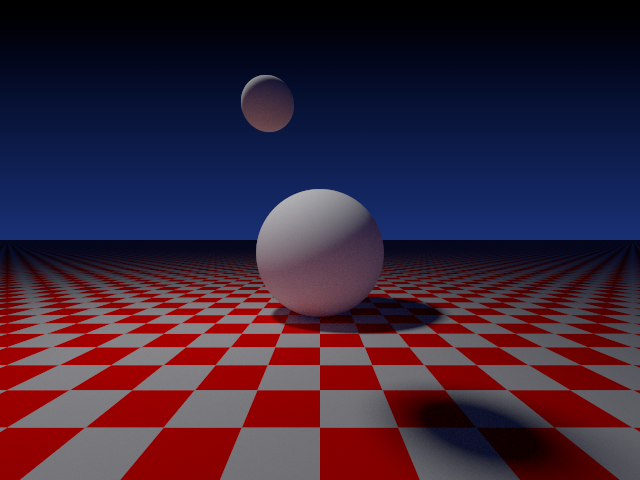
\includegraphics[width=0.5\textwidth]{exemplo_imagem}
%	\caption{
%		Um exemplo de uma imagem gerada utilizando \emph{path tracing}. Note como a luz que atinge o
%		plano xadrez é refletida de volta para iluminar a esfera, um fenômeno conhecido como
%		\emph{iluminação indireta} e que é corretamente simulado pelo algoritmo.
%	}
%	\label{fig:path_tracing}
%\end{figure}

\chapter{Desenvolvimento}

Aqui serão descritas as atividades realizadas para atingir os objetivos propostos. Essas atividades serão distribuídas em sessões de acordo com o segmento do projeto que mais se relacionam, sendo eles:

\begin{itemize}
	\item Ambiente de Desenvolvimento
	\item Organização do Projeto
	\item Modelos de dados
	\item Funcionalidades
	\item Design
	\item Administração
\end{itemize}

\section{Ambiente de Desenvolvimento}

\subsection{Sistema Operacional}

Para o desenvolvimento do projeto está sendo utilizado o sistema operacional Ubuntu 14.04(REF?), que contém um interpretador da linguagem Python(REF)?, sendo necessário apenas fazer a instalação do framework Django 1.8(REF?) para ter um ambiente pronto para começar o desenvolvimento do projeto. Além disso, também foi instalado o sistema de gerenciamento de pacotes pip(REF), que foi utilizado para instalação de outras ferramentas (descritas abaixo) que auxiliaram no desenvolvimento.

\subsection{Ferramentas de Programação}
Para auxiliar na tarefa de programação do sistema, foi utilizado o editor de texto Sublime Text 2 (REF!), um blabla.... utilizando também o plugin Anaconda... Django algo...

\subsection{Third Party Apps}
Falar dos pacotes que foram utilizados até agora, (Redux registration, Crispy, celery json-django)

\subsection{Controle de Versão - Repositório}

Para realizar o controle de versões foi utilizado o \emph{Git}\footnote{O repositório com o código pode ser encontrado em \url{https://github.com/Madalosso/TG}}, também utilizado pelo projeto original.

\section{Organização do Projeto}

O framework Django tem uma proposta de criar aplicações fáceis de serem reutilizadas por outros projetos, e por conta disso tem uma abordagem bastante metódica e pouco flexível em relação a distribuição dos arquivos que pertencem ao projeto. Consequentemente, a organização utilizada é a mesma proposta pela documentação do framework, que pode ser observada na figura abaix (incluir figura)

\subsection{\emph{manage.py}}
explicar a funcionalidade do manage e sua importancia para todo o projeto
\subsection{\emph{Static Files}}
explicar a opção de gerenciar arquivos estaticos (.css, .js e imgs utilizados nos templates)
\subsection{\emph{Templates}}
arquivos html 
\subsection{\emph{Media url}}
Explicar a organização do sistema de arquivos de entrada e saída dos experimentos (e o sistema de diretórios)
\subsection{\emph{settings.py}}
***falar com a Andrea e descobrir o quanto de texto eu devo abordar...****


\section{Modelos de dados}
adicionar imagem de algum software mostrando as relações entre os tipos de dados?
explicar o que cada classe / atributo tem como objetivo
\section{Funcionalidades}
Descvrever aqui as funcionalidades já implementadas ao sistema

\subsection{Administrador}
\subsection{Usuário registrado}
\subsection{Usuário Anonimo}
\section{Tasks}
Escrever como foi feito a manipulação e controle de tarefas (Celery).
\section{Design}
Explicar uso do Bootstrap,
jQuery,
tentativa de usar ajax e o porque não funcionou(por hora)
\section{Administração}
O que foi feito até então da parte de administração do sistema pelo administrador django
\iffalse

\begin{figure}
	\centering
	\begin{minipage}[t]{0.48\textwidth}
\begin{lstlisting}
enum Algorithm {
	kEyeLight,
	kPathTracing,
	kLightTracing,
	kProgressivePhotonMapping,
	kBidirectionalPhotonMapping,
	kBidirectionalPathTracing,
	kVertexConnectionMerging,
	kAlgorithmMax
};

static const char* GetName(Algorithm aAlgorithm) {
	static const char* algorithmNames[7] = {
		"eye light",
		"path tracing",
		"light tracing",
		"progressive photon mapping",
		"bidirectional photon mapping",
		"bidirectional path tracing",
		"vertex connection and merging"
	};

	if(aAlgorithm < 0 || aAlgorithm > 7)
		return "unknown algorithm";

	return algorithmNames[aAlgorithm];
}

static const char* GetAcronym(Algorithm aAlgorithm) {
	static const char* algorithmNames[7] = {
		"el", "pt", "lt", "ppm", "bpm", "bpt", "vcm" };

	if(aAlgorithm < 0 || aAlgorithm > 7)
		return "unknown";
	return algorithmNames[aAlgorithm];
}
\end{lstlisting}
	\end{minipage}
	~
	\begin{minipage}[t]{0.48\textwidth}
\begin{lstlisting}
enum Algorithm {
	EyeLight,
	PathTracing,
	LightTracing,
	ProgressivePhotonMapping,
	BidirectionalPhotonMapping,
	BidirectionalPathTracing,
	VertexConnectionMerging,
}

impl Algorithm {
	fn get_name(self) -> &'static str {
		match self {
			EyeLight => "eye light",
			PathTracing => "path tracing",
			LightTracing => "light tracing",
			ProgressivePhotonMapping => "progressive photon mapping",
			BidirectionalPhotonMapping => "bidirectional photon mapping",
			BidirectionalPathTracing => "bidirectional path tracing",
			VertexConnectionMerging => "vertex connection and merging",
		}
	}

	fn get_acronym(self) -> &'static str {
		match self {
			EyeLight => "el",
			PathTracing => "pt",
			LightTracing => "lt",
			ProgressivePhotonMapping => "ppm",
			BidirectionalPhotonMapping => "bpm",
			BidirectionalPathTracing => "bpt",
			VertexConnectionMerging => "vcm",
		}
	}
}
\end{lstlisting}
	\end{minipage}
	\caption{Comparação entre \emph{enums} em C++ e \emph{Rust}}
	\label{code:enums}
\end{figure}

Para a leitura de parâmetros passado via linha de comando, é utilizada o módulo \texttt{getopts} presente na biblioteca padrão. Na versão \Cpp\ a leitura é feita de forma manual.



\begin{figure}
\begin{lstlisting}
// Definição da macro
macro_rules! impl_Vector_traits(
	($Self:ident { $($field:ident),+ }) => (
		impl<T: Num> Add<$Self<T>, $Self<T>> for $Self<T> {
			#[inline]
			fn add(&self, o: &$Self<T>) -> $Self<T> {
				$Self {
					$($field: self.$field + o.$field),+
				}
			}
		}
		// ...
		impl<T: Num> Neg<$Self<T>> for $Self<T> {
			#[inline]
			fn neg(&self) -> $Self<T> {
				$Self {
					$($field: -self.$field),+
				}
			}
		}		
		// ...
		impl<T: Num> Index<uint, T> for $Self<T> {
			#[inline]
			fn index(&self, index: &uint) -> &T {
				[$(&self.$field),+][*index]
			}
		}
	)
)

// Definição dos tipos
#[deriving(Copy, Clone)]
pub struct Vector2<T> { pub x: T, pub y: T }
#[deriving(Copy, Clone)]
struct Vector3<T> { pub x: T, pub y: T, pub z: T }

// Instanciação da macro
impl_Vector_traits!(Vector2 { x, y })
impl_Vector_traits!(Vector3 { x, y, z })
\end{lstlisting}
\begin{lstlisting}
// Expansão de impl_Vector_traits!(Vector2 { x, y })
impl<T: Num> Add<Vector2<T>, Vector2<T>> for Vector2<T> {
	#[inline]
	fn add(&self, o: &Vector2<T>) -> Vector2<T> {
		Vector2 {
			x: self.x + o.x,
			y: self.y + o.y
		}
	}
}
// ...
impl<T: Num> Neg<Vector2<T>> for Vector2<T> {
	#[inline]
	fn neg(&self) -> Vector2<T> {
		Vector2 {
			x: -self.x,
			y: -self.y
		}
	}
}
// ...
impl<T: Num> Index<uint, T> for Vector2<T> {
	#[inline]
	fn index(&self, index: &uint) -> &T {
		[self.x, self.y][*index]
	}
}
\end{lstlisting}
	\caption{Definição e uso de uma macro e sua expansão}
	\label{code:mathmacro}
\end{figure}

I don't want this to happen
\fi
\chapter{Próximas Etapas}

Como continuação do trabalho realizado até o momento, são planejadas as seguintes atividades:

\begin{enumerate}
	\item fazer a execução das tarefas em uma máquina diferente da que mantém o portal.
	\item Avaliar novas idéias de funcionalidades e implementar as que forem validadas.
	\item tornar site responsivo via bootstrap.
\end{enumerate}

\setlength{\baselineskip}{\baselineskip}
\bibliographystyle{abnt}
\bibliography{../graphics,../languages}

\end{document}
